
\chapter{Tool Guide}

\section{Git}

\subsubsection{Revert to the previous commit}
From the repository directory in Git Bash or the PhpStorm Terminal enter:\\

\begin{tabular}{l}
	\texttt{git reset --hard HEAD}\\
\end{tabular}

\begin{quote}
	\emph{Warning! This will erase any and all uncommitted changes!}
\end{quote}

\subsubsection{Create a new local branch}

\subsubsection{Add a local branch to remote}
From the repository directory in Git Bash or the PhpStorm Terminal enter:\\
\\
\begin{tabular}{l}
	\texttt{git push -u origin $<$Branch Name$>$}
\end{tabular}
\section{Gerrit}
\label{sec:Gerrit}

Gerrit is a web based code review system, facilitating online code reviews for projects using the Git version control system.

Gerrit makes reviews easier by showing changes in a side-by-side display, and allowing inline comments to be added by any reviewer.

\subsection{Workflow}

\begin{figure}[H] 
	\centering
	\vspace{3pt}
	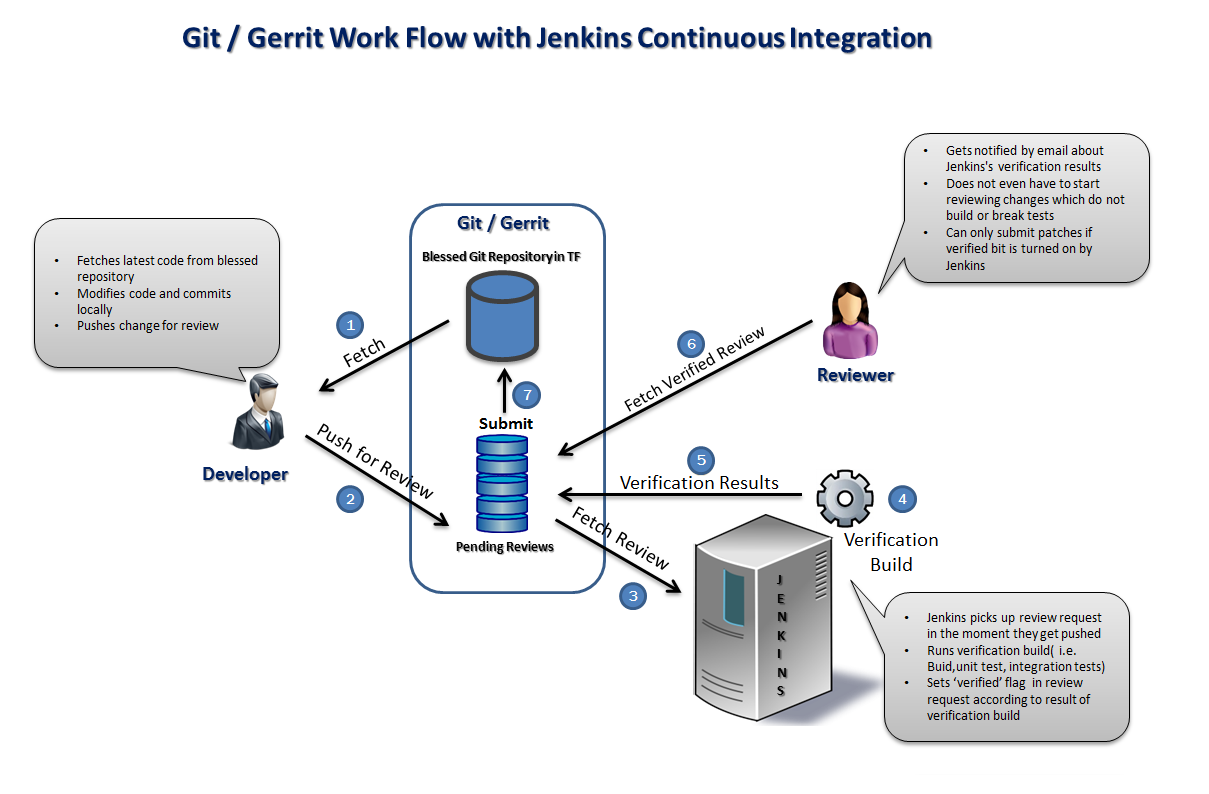
\includegraphics[width=12cm]{Git_gerrit_jenkins}
	\caption{Git Gerrit Jenkins Workflow}
\end{figure}


\subsection{Cloning repository}
In order to clone a repository to your local computer look at section \ref{subsec:Core_library} \footnote{\ref{subsec:Core_library} THM Core Library}.

\subsection{Push to repository} 
After working on the project we need to push our changes back to gerrit. To do so just rightclick the project and select Git -- Commit Directory...

\begin{figure}[H] 
	\centering
	\vspace{3pt}
	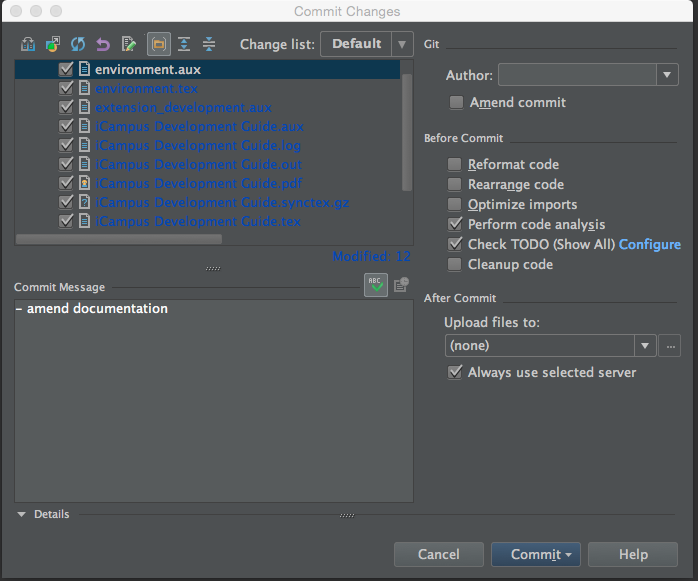
\includegraphics[width=7cm]{gerrit-commit-directory.png}
	\caption{Gerrit Commit Directory}
\end{figure}

\textbf{Please watch out!} If you want to recommit a modification depending the same change, be sure to check the Amend commit Checkbox. This will not lead to a new Changeset but in an update of your precommitted change. Do not delete old Commit-Message. Just amend the message.

\begin{figure}[H] 
	\centering
	\vspace{3pt}
	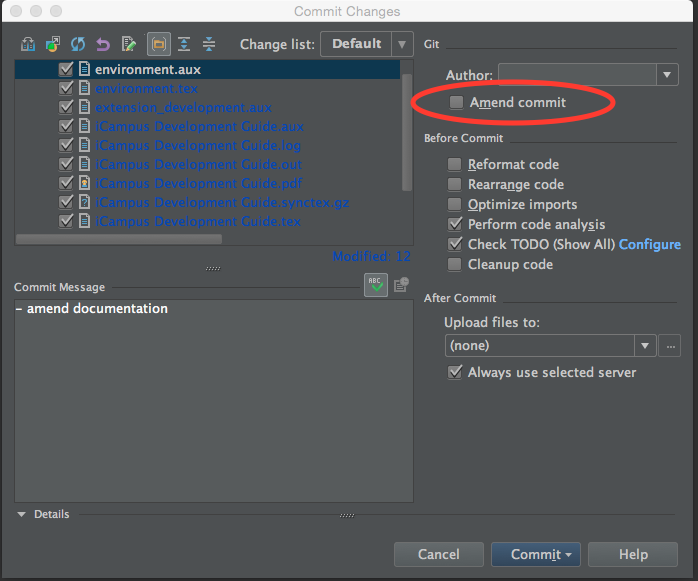
\includegraphics[width=7cm]{gerrit-commit-directory-amend}
	\caption{Gerrit Amend Commit}
\end{figure}

After we committed the change with a useful comment, we need to push it to Gerrit. In spite we have the latest version of the Gerrit plugin in PhpStorm we just need to rightclick the project and select Git -- Push and check "Push to Gerrit". It is possible to declare reviewers who will be informed about the push.

\begin{figure}[H] 
	\centering
	\vspace{3pt}
	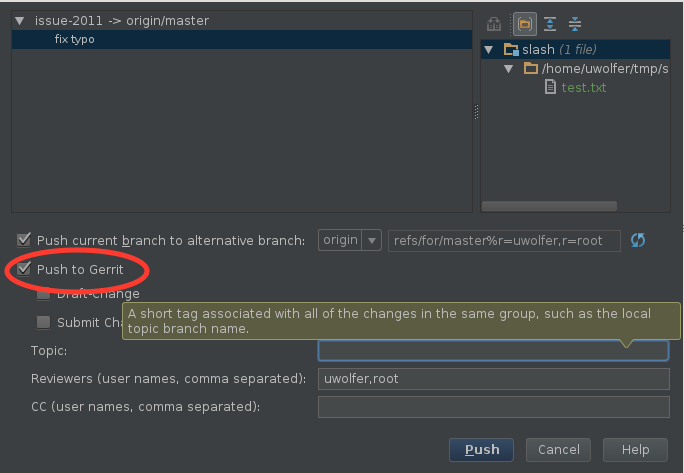
\includegraphics[width=8cm]{gerrit-push-new}
	\caption{Gerrit Push New}
\end{figure}

If the Plugin is not at its latest version we have to push to a specific branch. Please check the box at "Push current branch to alternate branch" and type the following in the textbox: "refs/for/master". We should not be able to push to any other branch except we are the projectowner. 

\begin{figure}[H] 
	\centering
	\vspace{3pt}
	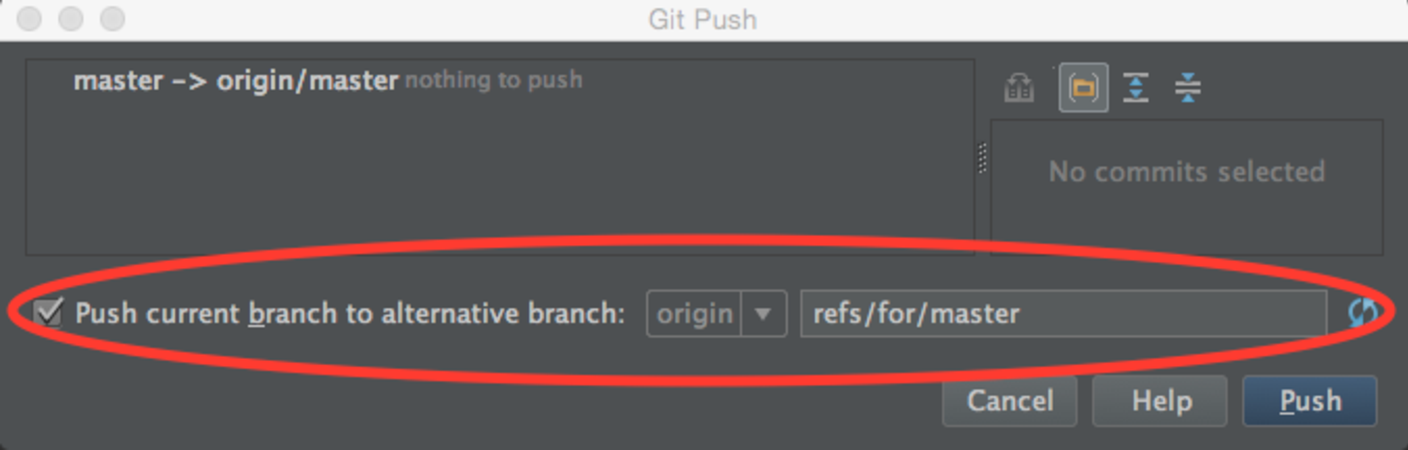
\includegraphics[width=8cm]{gerrit-push-old}
	\caption{Gerrit Push Old}
\end{figure}

Afterwards we should be able to see the change in the gerrit window of our PhpStorm installation.

\subsection{Review change}
The Gerrit Tool Window\footnote{\ref{subsec:Tool-window-activation} Tool Window Activation} will show us all changes for the project we are working on. We have access on different actions like review, submit...

\begin{figure}[H] 
	\centering
	\vspace{3pt}
	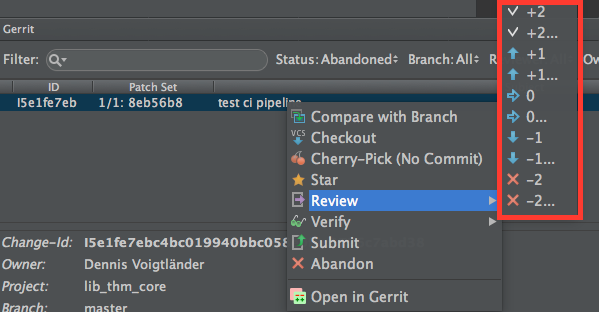
\includegraphics[width=8cm]{gerrit-review}
	\caption{Gerrit Review Scores}
\end{figure}

A change has to have a minimum Review-Score of +2 in order to be merged into master. The change also has to be verified by jenkins. Only the projectowner is authorized the merge the change into master. He can do it by clicking on the change and choose "Submit".

\subsection{Submit/Abandon change}
Submitting a change in Gerrit means that a attached change gets merged into master (only possible for projectowner). Therefor a release will be created. The projectowner can  rightclick a change and choose "Submit" if the cahnge should be released as a patch. It will only succeed if the change is reviewed with a minimum score of +2 and if its verified +1 by jenkins. If the change should be released as a feature, the projectowner needs to visit the Webinterface\footnote{\url{http://www.gerrit.mni.thm.de/gerrit}} of Gerrit and type in the topic of the change "feature" before he submits (until now - will also be able in IDE in near future). 

\begin{figure}[H] 
	\centering
	\vspace{3pt}
	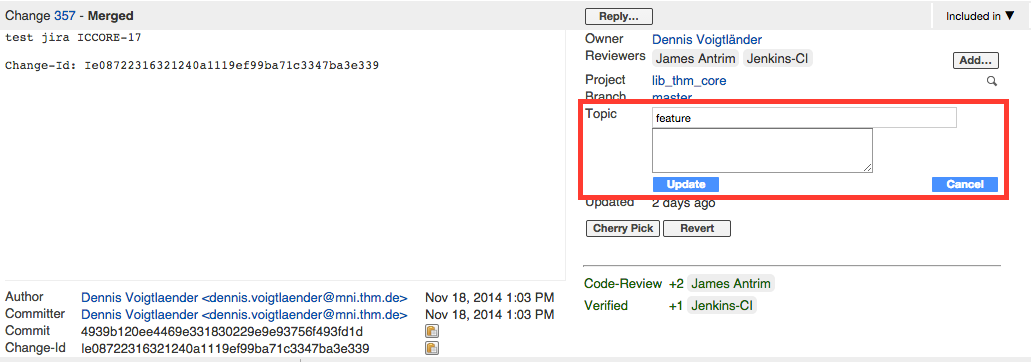
\includegraphics[width=10cm]{gerrit-feature}
	\caption{Gerrit Feature}
\end{figure}

If nothing is declared in the textbox topic, the change will be released as a patch.


